\begin{figure}[h!]
	\centering
	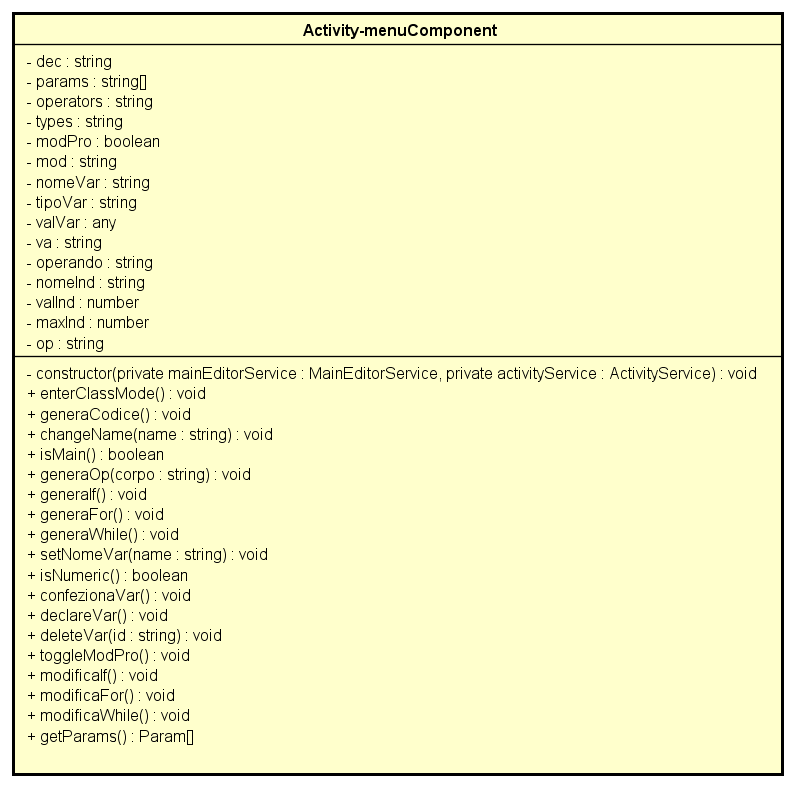
\includegraphics[scale=0.8]{res/sections/SpecificaFrontEnd/Components/Disegnetti/activity-menu.png}
	\caption{Diagramma della classe Activity-menu}
\end{figure}

\begin{itemize}
	
	\item \textbf{Descrizione:}\\
	
	\item \textbf{Utilizzo:}\\
	
	\item \textbf{Attributi:}
		\begin{itemize}
			\item \emph{-decisions: string[]}\\
			Lista delle decisioni
			\item \emph{-dec: string}\\
			Decisione presa
			\item \emph{-params: string[]}\\
			Lista dei parametri
			\item \emph{-operators: string}\\
			Lista degli operatori
			\item \emph{-types: string}\\
			Lista dei tipi
			\item \emph{-modPro: boolean}\\
			Modalità del body
			\item \emph{-mod: string}\\
			Assegna un bottone in html DOM
			\item \emph{-nomeVar: string}\\
			Nome della variabile
			\item \emph{-tipoVar: string}\\
			Tipo della variabile
			\item \emph{-valVar: any}\\
			Valore della variabile
			\item \emph{-va: string}\\
			Nome della variabile dell'if statement
			\item \emph{-operando: string}\\
			Operando dell'if
			\item \emph{-nomeInd: string}\\
			Nome della variabile per il loop
			\item \emph{-valInd: number}\\
			Variabile indice per il loop
			\item \emph{-maxInd: number}\\
			Indice massimo per il loop
			\item \emph{-op: string}\\
			Operazione
		\end{itemize}
	\item \textbf{Metodi:}
		\begin{itemize}
			\item \emph{-constructor(private mainEditorService: MainEditorService,
		private activityService: ActivityService)}\\
    		Costruttore della classe\\
    		\textbf{Parametri:}
    		\begin{itemize}
    			\item \emph{mainEditorService: MainEditorService}\\
    			Crea un istanza di MainEditorService
    			\item \emph{activityService: ActivityService}\\
    			Crea un istanza di ActivityService
    		\end{itemize}
    		\item \emph{+enterClassMode()}\\
    		Entra nel diagramma delle classi
    		\item \emph{+generaCodice()}\\
    		Genera il codice
    		\item \emph{+changeName(name: string)}\\
    		Cambia il nome con un nuovo valore\\
    		\textbf{Parametri:}
    		\begin{itemize}
    			\item \emph{name: string}\\
    			Nuovo nome
    		\end{itemize}
    		\item \emph{+isMain()}\\
    		Ritorna true se il metodo è main
    		\item \emph{+generaOp(corpo: string)}\\
    		Genera il corpo dell'operazione\\
    		\textbf{Parametri:}
    		\begin{itemize}
    			\item \emph{corpo: string}\\
    			Corpo dell'operazione
    		\end{itemize}
    		\item \emph{+generaIf()}\\
    		Genera l'if statemente
    		\item \emph{+generaFor()}\\
    		Genera il ciclo for
    		\item \emph{+generaWhile()}\\
    		Genera il ciclo while
    		\item \emph{+setNomeVar(name: string)}\\
    		Setta il nuovo nome della variabile\\
    		\textbf{Parametri:}
    		\begin{itemize}
    			\item \emph{name: string}\\
    			Nuovo nome della variabile
    		\end{itemize}
    		\item \emph{+isNumeric()}\\
    		Ritorna true se la stringa è numerica
    		\item \emph{+confezionaVar()}\\
    		La funzione costruisce la variabile
    		\item \emph{+declareVar()}\\
    		Dichiara la variabile
    		\item \emph{+deleteVar(id: string)}\\
    		Elimina una variabile\\
    		\textbf{Parametri:}
    		\begin{itemize}
    			\item \emph{id: string}\\
    			Id della variabile da eliminare
    		\end{itemize}
    		\item \emph{+toggleModPro()}\\
    		Modifica il modo per editare uno statement
    		\item \emph{+modificaIf()}\\
    		Edita l'if statement
    		\item \emph{+modificaFor()}\\
    		Edita il ciclo for
    		\item \emph{+modificaWhile()}\\
    		Edita il ciclo while
    		\item \emph{+getParams()}\\
    		Ritorna la lista dei parametri
		\end{itemize}
\end{itemize}